%
% Vorlage für Versuchsprotokolle im Grundpraktikum an der RWTH Aachen
% -------------------------------------------------------------------
%
% Bitte verwenden Sie diese Vorlage zur Erstellung Ihrer
% Protokolle.
%
% Wenn möglich, drucken Sie Ihre Protokolle bitte doppelseitig
% aus. Wenn Sie das Protokoll doppelseitig ausdrucken, verwenden Sie
% die twoside Option ...
\documentclass[twoside]{protokoll}
% ... wenn Sie nicht doppelseitig ausdrucken können, lassen Sie sie
% weg:
%\documentclass{protokoll}

% Setzen Sie hier "I" für den Teil 1 oder "II" für den Teil 2 ein:
\praktikum{I}
 
% Setzen Sie hier das jeweilige Versuchsgebiet ein (Mechanik,
% Akustik, Thermodynamik, Elektrizitätslehre, usw.):
\versuchsgebiet{(Gebiet)}

% Setzen Sie hier Ihren Namen und Ihre Matrikelnummer sowie Ihre
% Gruppennummer ein (ohne die Klammern):
\teilnehmer{Name 1. Teilnehmer, (Matrikelnummer)}
\teilnehmer{Name 2. Teilnehmer, (Matrikelnummer)}
\gruppe{(Gruppennummer)}

\begin{document}

% Ersetzen Sie den folgenden Text durch eine kurze Beschreibung der
% Versuchsziele.
\begin{versuchsziele}
  Kurze Beschreibung der Versuchsziele aller Teilversuche.
\end{versuchsziele}

%
% Hier werden die bearbeiteten Aufgaben ausgewählt, indem das
% Prozentzeichen (%) vor dem jeweiligen \input-Befehl entfernt
% wird. Die tex-Dateien können im Moodle in den entsprechenden
% Unterordnern bei den einzelnen Versuchsgebieten heruntergeladen
% werden. Achten Sie darauf, dass sich alle benötigten Dateien im
% selben Verzeichnis befinden, bevor Sie diese tex-Datei kompilieren.
%
% Die Bearbeitung der Aufgaben findet unmittelbar in der jeweiligen
% Datei ("aufgaben_xXy.z.tex") statt. Dort befinden sich Umgebungen
% der Form
%
% \begin{aufgabe}
%   ... (Hinweise) ... bzw.
%   ... (Aufgabentext) ...
% \end{aufgabe}
%
% Allgemeine Hinweise entfernen Sie bitte. Hinter dem
% versuchsspezifischen Aufgabentext und dem "\end{aufgabe}" beginnen
% Sie Ihre Lösung der Aufgabe.
%

%
% Grundpraktikum Teil I
%

% Mechanik
%\section{1M1 Messung der Erdbeschleunigung mit dem Pendel}

\begin{aufgabe}{Grundlagen}
  Knappe Beschreibung der theoretischen Grundlagen, Angabe der
  benötigten Formel(n), ohne Herleitung. Definition der verwendeten
  Formelzeichen.
\end{aufgabe}

% Bitte belassen Sie die Aufgabentexte in Ihrem Protokoll und beginnen
% Sie hier mit der Lösung der ersten Aufgabe:



\begin{aufgabe}{Versuchsaufbau und Versuchsdurchführung}
  Beschreibung des Versuchsaufbaus einschließlich beschrifteter Skizze
  oder Foto. Beschreibung der Versuchsdurchführung: Handgriffe an der
  Apparatur, verwendete Messwerterfassungseinstellungen, Messbereiche,
  Triggerbedingungen, etc.
\end{aufgabe}


\begin{aufgabe}{Rohdaten}
  Stellen Sie Ihre Rohdaten dar, tabellarisch für $l_p$ und $r_p$,
  grafisch für den Verlauf der Schwingung der Stange ohne Pendelkörper
  sowie der Pendelschwingung (für mindestens drei Messreihen).
\end{aufgabe}


\begin{aufgabe}{Auswertung}
  Bestimmen Sie für alle Messreihen die Periodendauer und ihre
  Messunsicherheit, indem Sie eine geeignete lineare Regression
  durchführen. Demonstrieren Sie, dass Sie das Trägheitsmoment der
  Stange kompensiert haben. Tabellieren Sie die Zwischenergebnisse
  der relevanten Größen samt ihrer Messunsicherheiten. Berechnen
  Sie die Erdbeschleunigung. Führen Sie eine Fehlerrechnung zur
  Bestimmung der Messunsicherheit durch. Geben Sie bei Ihrer
  Fehlerrechnung die Größe der Einzelbeiträge an, die zu dem
  Gesamtfehler führen. Diskutieren Sie, welcher Fehler den
  Gesamtfehler dominiert. Vergleichen Sie Ihr Endergebnis mit dem
  relevanten Literaturwert.
\end{aufgabe}




%\input{aufgaben_1M2.tex}
%\input{aufgaben_1M4.tex}

% Akustik
%\input{aufgaben_1A1.tex}
%\input{aufgaben_1A2.tex}
%\section{1A3 Bestimmung des E-Moduls von Metallen}

\begin{aufgabe}{Grundlagen}
  Knappe Beschreibung der theoretischen Grundlagen, Angabe der
  benötigten Formel(n), ohne Herleitung. Definition der verwendeten
  Formelzeichen.
\end{aufgabe}

% Bitte belassen Sie die Aufgabentexte in Ihrem Protokoll und beginnen
% Sie hier mit der Lösung der ersten Aufgabe:



\begin{aufgabe}{Versuchsaufbau und Versuchsdurchführung}
  Beschreibung des Versuchsaufbaus einschließlich beschrifteter Skizze
  oder Foto. Beschreibung der Versuchsdurchführung: Handgriffe an der
  Apparatur, verwendete Messwerterfassungseinstellungen, Messbereiche,
  Triggerbedingungen, etc.
\end{aufgabe}


\begin{aufgabe}{Rohdaten}
  Stellen Sie die gemessenen Werte von $L$, $D$ und $M$ in
  tabellarischer Form dar. Visualisieren Sie einige typische
  Schwingungsverläufe sowie deren Fourierspektren in geeigneter
  Weise.
\end{aufgabe}


\begin{aufgabe}{Auswertung}
  Bestimmen Sie aus den aufgezeichneten Schwingungsvorgängen die
  Schwingungsfrequenzen und tabellieren Sie die erhaltenen
  Werte. Ermitteln Sie die Streuung der einzelnen $f_i$ und bestimmen
  Sie daraus den statistischen Fehler auf den Mittelwert. Erläutern
  und illustrieren Sie Ihr Vorgehen zur Bestimmung der systematischen
  Unsicherheiten auf die Frequenz. Diskutieren Sie die Unsicherheiten
  auf $L$, $D$ und $M$. Berechnen Sie den E-Modul und die Dichte der
  vorliegenden Stangen und die zugehörigen statistischen und
  systematischen Messunsicherheiten. Diskutieren Sie, welche
  Fehlerbeiträge den Gesamtfehler dominieren. Vergleichen Sie Ihre
  Ergebnisse mit einschlägigen Literaturwerten.
\end{aufgabe}




%\input{aufgaben_1A4.tex}


% Wärmelehre
%
%\input{aufgaben_1T1.tex}
%\input{aufgaben_1T2.tex}
%\input{aufgaben_1T3.tex}

% Elektrizitätslehre
%
%\section{1E1 Ladekurven eines Kondensators}

\begin{aufgabe}{Grundlagen}
  Knappe Beschreibung der theoretischen Grundlagen, Angabe der
  benötigten Formel(n), ohne Herleitung. Definition der verwendeten
  Formelzeichen.
\end{aufgabe}

% Bitte belassen Sie die Aufgabentexte in Ihrem Protokoll und beginnen
% Sie hier mit der Lösung der ersten Aufgabe:



\begin{aufgabe}{Vorversuch: Charakterisierung der verwendeten Bauteile}
  Charakterisieren Sie die verwendeten Bauteile mit Digitalvoltmeter
  und Messbrücke.
\end{aufgabe}


\begin{aufgabe}{Vorversuch: Bestimmung des Ohmschen Widerstands}
  Beschreiben Sie den Versuchsaufbau unter Verwendung eines
  Schaltbildes. Beschreiben Sie die Versuchsdurchführung unter Angabe
  der relevanten Messwerterfassungseinstellungen. Zeigen Sie
  exemplarisch die Häufigkeitsverteilungen für Spannung $U$ und Strom
  $I$ an einem Messpunkt und beschreiben Sie, wie Sie die
  statistischen Fehler für $U$ und $I$ bestimmen. Tragen Sie die
  Spannung $U$ gegen den Strom $I$ auf und bestimmen Sie aus der
  Steigung den Widerstand $R$ und seine statistische
  Messunsicherheit. Ermitteln Sie den systematischen Fehler mit der
  Verschiebemethode.
\end{aufgabe}


\begin{aufgabe}{Lade- und Entladekurven des Kondensators mit dem Oszilloskop}
  Beschreiben Sie den Versuchsaufbau unter Verwendung eines
  Schaltbildes. Beschreiben Sie die Versuchsdurchführung unter Angabe
  der relevanten Messwerterfassungseinstellungen. Zeigen Sie für den
  Lade- und den Entladevorgang jeweils ein Bild der gemessenen
  Spannungsverläufe auf dem Oszilloskopschirm. Lesen Sie mithilfe der
  Cursor jeweils die Zeitkonstante ab. Berechnen Sie den gewichteten
  Mittelwert der Zeitkonstanten. Berechnen Sie daraus die Kapazität
  und geben Sie sie mit statistischer und systematischer
  Messunsicherheit an.
\end{aufgabe}


\begin{aufgabe}{Lade- und Entladekurven des Kondensators mit Cassy}
  Zeigen Sie für den Lade- und den Entladevorgang jeweils ein Bild des
  Spannungsverlaufs am Kondensator und des Lade- bzw.~Entladestroms.
  Korrigieren Sie erforderlichenfalls den Spannungs- und/oder
  Strom-Offset. Transformieren Sie die Rohdaten geeignet in
  logarithmische Größen und bestimmen Sie mittels linearer Regression
  die Zeitkonstante. Beschreiben Sie, wie Sie die Messunsicherheiten
  behandeln. Berechnen Sie das gewichtete Mittel und geben Sie Ihr
  Endergebnis für die Kapazität mit statistischer und systematischer
  Messunsicherheit an.
\end{aufgabe}


\begin{aufgabe}{Zusammenfassung und Diskussion}
  Fassen Sie Ihre Ergebnisse zu den Kapazitäten zusammen und
  vergleichen Sie sie untereinander, mit den Messungen aus dem
  Vorversuch und mit den Herstellerangaben (Toleranz
  $\SI{5}{\percent}$).  
\end{aufgabe}


%\input{aufgaben_1E2.tex}
%\section{1E3 Gekoppelte LC-Schwingkreise}

\begin{aufgabe}{Grundlagen}
  Knappe Beschreibung der theoretischen Grundlagen, Angabe der
  benötigten Formel(n), ohne Herleitung. Definition der verwendeten
  Formelzeichen.
\end{aufgabe}

% Bitte belassen Sie die Aufgabentexte in Ihrem Protokoll und beginnen
% Sie hier mit der Lösung der ersten Aufgabe:



\begin{aufgabe}{Versuchsaufbau und Versuchsdurchführung}
  Beschreibung des Versuchsaufbaus einschließlich
  Schaltbild. Beschreibung der Versuchsdurchführung: verwendete
  Messwerterfassungseinstellungen, Messbereiche, Triggerbedingungen,
  etc.
\end{aufgabe}


\begin{aufgabe}{Vorversuch: Charakterisierung der verwendeten Bauteile}
  Charakterisieren Sie die verwendeten Bauteile mit Digitalvoltmeter
  bzw. Messbrücke.
\end{aufgabe}


\begin{aufgabe}{Ungekoppelte Schwingung}
  Zeigen Sie den Verlauf der Kondensatorspannungen für den
  ungekoppelten Fall und bestimmen Sie die Schwingungsfrequenz samt
  Messunsicherheit. Vergleichen Sie sie mit Ihrer Erwartung.
\end{aufgabe}


\begin{aufgabe}{Gekoppelte Schwingung: Schwebung}
  Stellen Sie für einen festen Kopplungsgrad $k$ eine Schwebung
  dar. Zeigen Sie jeweils die Fourierspektren, bestimmen Sie die
  Eigenfrequenzen und daraus den Kopplungsgrad sowie dessen
  Messunsicherheit. Bestimmen Sie die zeitliche Verschiebung
  $\Delta{}t$ zwischen den beiden Einhüllenden der Schwebungen der
  beiden Kondensatoren und vergleichen Sie sie mit Ihrer
  Erwartung. Stellen Sie dar, wie sich das Frequenzspektrum mit dem
  Abstand der Spulen ändert. Untersuchen Sie die Verstärkung der
  Kopplung durch Verwendung eines Eisenkerns in den beiden Spulen.
\end{aufgabe}


\begin{aufgabe}{Gekoppelte Schwingung: gleich- und gegensinnige Anregung}
  Stellen Sie für einen festen Kopplungsgrad $k$ nacheinander die
  beiden Fundamentalschwingungen dar. Zeigen Sie jeweils die
  Fourierspektren und bestimmen Sie die zugängliche
  Eigenfrequenz. Berechnen Sie den Kopplungsgrad sowie dessen
  Messunsicherheit. Vergleichen Sie mit den Werten aus der Schwebung.
\end{aufgabe}



%
% Grundpraktikum Teil II
%

% Atomphysik
%\input{aufgaben_2A1.tex}

% Optik I
%\input{aufgaben_2O1.tex}

% Optik II
%\input{aufgaben_2O3.tex}

% Elektrizitätslehre (Teil II)
%
%\input{aufgaben_2E1.tex}


%
% Der nachfolgende Abschnitt mag nützlich sein, um Vorlagen für häufig
% vorkommende Arbeitsschritte mit LaTeX daraus zu entnehmen. Er muss
% vor Abgabe des Protokolls entfernt werden. (Das \end{document} muss
% aber natürlich erhalten bleiben.)
%
\clearpage
\section*{Grundlagen von \LaTeX}
Hier sollen die wichtigsten Grundlagen von \LaTeX{} knapp rekapituliert
werden, die typischerweise bei der Erstellung eines
Praktikumsprotokolls benötigt werden. Sie können die Beispiele aus
diesem Abschnitt als Vorlage für Ihre eigenen Protokolle
verwenden. Für eine tiefergehende Dokumentation sei auf die Literatur
verwiesen, wobei zu Beginn insbesondere die folgenden Quellen
hilfreich sein können:
\begin{enumerate}
\item T.~Oetiker, Not so short Introduction to \LaTeX,
  \url{www.ctan.org/tex-archive/info/lshort/german/l2kurz.pdf}.
\item Dokumentation, die von der Overleaf-Plattform frei zugänglich
  zur Verfügung gestellt wird: \url{www.overleaf.com/learn}.
\end{enumerate}

\subsection*{Formeln}
Einfache Formeln wie $s=vt$ können direkt im Text gesetzt
werden. Wichtige oder kompliziertere Gleichungen werden mittels einer
\texttt{equation}-Umgebung gesetzt:
\begin{equation}
  \label{eq:fehlerrechnung}
  \left(\frac{\sigma_s}{s}\right)^2 =
  \left(\frac{\sigma_v}{v}\right)^2 +
  \left(\frac{\sigma_t}{t}\right)^2.
\end{equation}
Über Referenzen kann man dann einfach auf die entsprechende
Gleichung~(\ref{eq:fehlerrechnung}) verweisen.

\subsection*{Einheiten}
Um einheitenbehaftete Größen korrekt zu setzen, wird das Paket
\href{https://ctan.org/pkg/siunitx?lang=de}{\texttt{siunitx}}
verwendet. Beispiele finden sich in folgendem Satz: ``Das Pendel hat
eine Länge von \SI{1.5}{m} bei einer Temperatur von
$T=\SI{20}{\degreeCelsius}$. Das führt zu einem Ergebnis von
$g=\SI{9.81+-0.01}{m.s^{-2}}$.''

\subsection*{Abbildungen}
Abbildungen lassen sich mit einer \texttt{figure}-Umgebung
einfügen. Verweise (Abb.~\ref{fig:beispiel}) lassen sich dann
automatisch in den Text einbinden. Wählen Sie für den Export von
Abbildungen das richtige Dateiformat: Für Darstellungen am Bildschirm,
also z.B.~für Vorträge, werden Pixelgrafiken benötigt. Hierfür bietet
sich insbesondere das \texttt{png}-Format an, bei dem die Bilddaten
verlustfrei komprimiert werden. Für Abbildungen im Protokoll
exportiert man die Plots als Vektorgrafik, denn diese lässt sich
beliebig skalieren. Man verwendet am besten das \texttt{pdf}-Format,
weil es sich direkt mit \texttt{pdflatex} verarbeiten
lässt. (Ausnahme: Plots mit sehr vielen Datenpunkten ($>10000$)
bringen den Moodle-Lernraum zum Absturz und sollen als \texttt{png}
abgespeichert werden.) Fotos u.ä.~können direkt im \texttt{jpg}-Format
eingebunden werden. Für Plots ist das \texttt{jpg}-Format aber
keinesfalls geeignet, weil dann regelmäßig stakre
Kompressionsartefakte auftreten.
\begin{figure}[t]
  \centering
  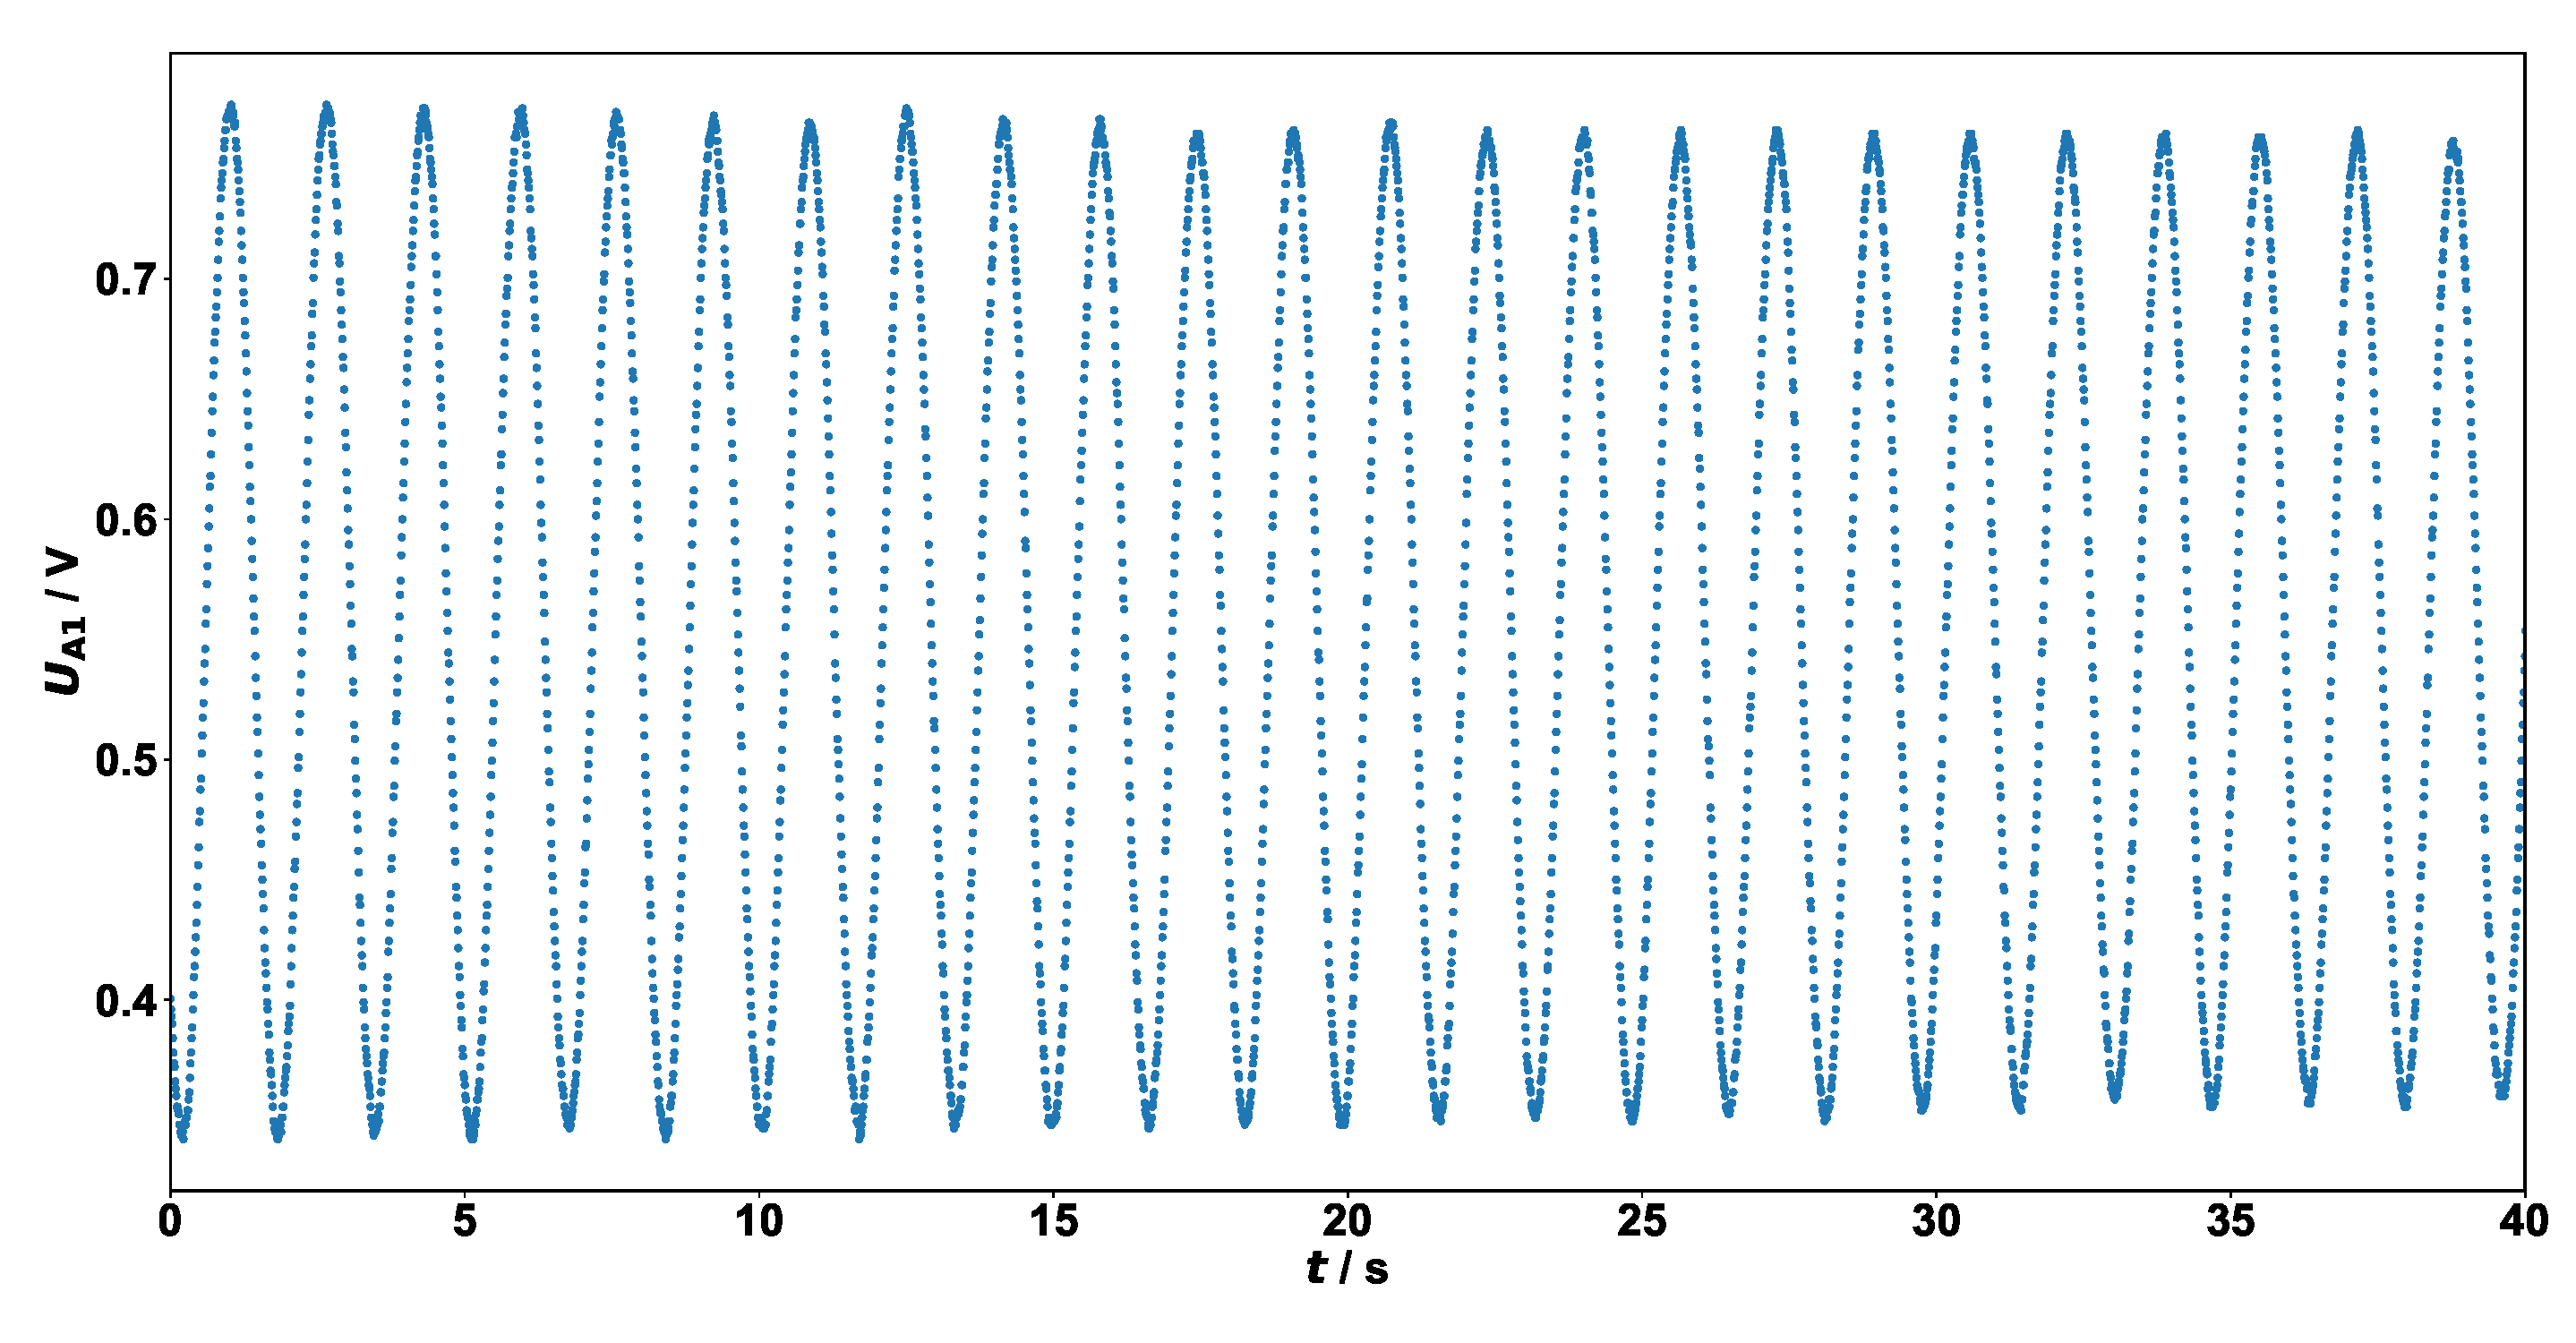
\includegraphics[width=0.95\textwidth]{beispiel_abbildung.pdf}
  \caption{Beispiel für eine Abbildung. In der Bildunterschrift
    sollten alle Informationen enthalten sein, die für das Verständnis
    der Abbildung benötigt werden. Die Interpretation des gezeigten
    findet dann aber im Text statt.}
  \label{fig:beispiel}
\end{figure}

\subsection*{Tabellen}
Tabellen werden mit der \texttt{tabular}-Umgebung gesetzt, die sich
innerhalb einer \texttt{table}-Umgebung befindet, wie im Beispiel von
Tabelle~\ref{tab:beispieltabelle}.
\begin{table}[h]
  \centering
  \begin{tabular}{l|ccc}
    Position $S$ (cm) & \multicolumn{3}{|c}{Laufzeiten $t$ (ms)} \\ \hline
     2,0 & 0,8943 & 0,8944 & 0,8943 \\
         & 0,8953 & 0,8945 & 0,8942 \\ \hline
     6,0 & 0,9921 & 0,9912 & 0,9923 \\
         & 0,9922 & 0,9902 & 0,9929 \\ \hline
    10,0 & 1,0988 & 1,0977 & 1,0982 \\
         & 1,0991 & 1,0992 & 1,0993 \\ \hline
  \end{tabular}
  \caption{Beispieltabelle.}
  \label{tab:beispieltabelle}
\end{table}

\subsection*{Einstellungen}
Um Messwerterfassungseinstellungen und ähnliches kompakt
zusammenzustellen, eignet sich die \texttt{verbatim}-Umgebung:
\begin{verbatim}
Kanal A: Einstellungen
Kanal B: Einstellungen
Messparameter: ...
\end{verbatim}

\subsection*{Protokoll setzen}
Um aus den \LaTeX{}-Quellen eine pdf-Datei zu erzeugen, verwendet man
unter Linux am einfachsten den folgenden Befehl:
\begin{verbatim}
  latexmk -pdf Protokoll
\end{verbatim}

\noindent Dabei ist \texttt{Protokoll} durch den jeweiligen Dateinamen zu
ersetzen, die Endung \texttt{.tex} kann weggelassen werden.

%
% Es folgen Checklisten, mit denen man die häufigsten Fehler bei
% typischen Arbeitsschritten im Praktikum vermeiden kann. Bitte vor
% Abgabe des Protokolls entfernen!
%
\clearpage
\section*{Checklisten}
Es folgen Checklisten, mit denen man die häufigsten Fehler bei
typischen Arbeitsschritten im Praktikum vermeiden kann. Bitte vor
Abgabe des Protokolls entfernen!

\subsection*{Diagramme}
\begin{checklist}
\item Achsenbeschriftungen vollständig mit Größe und Einheit?
\item Wertebereich in $x$- und $y$-Richtung sinnvoll gewählt?
\item Ausreichende Schriftgröße für alle Beschriftungen?
\item Ausreichende Liniendicke, Symbolgröße, etc.?
\item Aussagekräftige Bildunterschrift hinzugefügt?
\item Aussagekräftige Legende, falls notwendig?
\item Abbildung in ausreichender Größe im Protokoll eingebunden?
\item Richtiges Dateiformat gewählt? In aller Regel Vektorgrafik: eps
  oder pdf, Ausnahme: Plots mit sehr vielen Datenpunkten ($>10000$),
  diese bringen den Moodle-Lernraum zum Absturz und sollen als png
  eingebunden werden.
\item Verweis auf Abbildung im Text eingefügt? Auf jede Abbildung muss
  im laufenden Text verwiesen werden.
\end{checklist}

\noindent In aller Regel werden Messdaten in Form von kreisförmigen Markern,
ggfs.~mit Fehlerbalken, eingetragen, Modellanpassungen u.ä.~dagegen in
Form von Linien bzw.~Kurven. Lediglich wenn sehr viele Messpunkte
vorliegen, kann es angemessen sein, statt einzelner Punkte eine alle
Messpunkte verbindende Linie einzuzeichnen.

\subsection*{Regressionsanalyse}
\begin{checklist}
\item Aussagekräftiges Diagramm (s.o.)?
\item Fehler auf Einzelpunkte, in $y$- und ggfs.~in $x$-Richtung
  diskutiert?
\item Diejenige Größe mit den kleineren relativen Unsicherheiten auf
  der $x$-Achse aufgetragen?
\item Residuenplot entsprechend des Beispiels aus der
  Praktikumsbibliothek hinzugefügt und korrekt beschriftet?
\item $\chi^2/dof$ angegeben, und zwar getrennt und im Verhältnis, in
  der Form $\chi^2/dof=24/20=1.2$?
\item Möglicherweise erkennbare systematische Abweichungen von der
  Modellkurve diskutiert?
\end{checklist}

\subsection*{Fourieranalyse}
\begin{checklist}
\item Abtastrate und Dauer der Messung geschickt gewählt?
\item Im Fourierspektrum ggfs.~den Ausschnitt der Frequenzachse so
  angepasst, dass Form und Breite von Peaks gut beurteilt werden
  können?
\item Statistische Messunsicherheit der Peakposition durch
  Wiederholungsmessung bestimmt? Behelfsweise Abschätzung, wie genau
  die Lage des Peaks besimmt werden kann.
\end{checklist}

\subsection*{Ergebnisse}
\begin{checklist}
\item Endergebnisse angegeben und klar als solche kenntlich gemacht?
\item Endergebnisse mit Einheit sowie statistischer und
  ggfs.~systematischer Messunsicherheit angegeben?
\item Nur signifikante Stellen angegeben?
\item Vergleich mit Literaturwert oder Herstellerangabe?
\item Ggfs.~Vergleich von Ergebnissen, die mit verschiedenen Methoden
  gewonnen wurden, durchgeführt?
\end{checklist}

\subsection*{Protokollabgabe}
\begin{checklist}
\item Alle Aufgaben bearbeitet? (Es sollen keine Aufgaben ausgelassen
  werden.)
\item Versuchsdurchführung: Verwenden Sie die 1. Person im Perfekt
  Indikativ (\glqq{}wir haben darauf geachtet\grqq{}, nicht aber
  \glqq{}man sollte darauf achten\grqq{})?
\item Auswertung: Vorgehen nachvollziehbar beschrieben? Verwendete
  Formeln (insbesondere zur Fehlerrechnung) und relevante
  Zwischenergebnisse angegeben?
\item Alle Dateien gemäß der vorgegebenen Konvention benannt?\newline
  D.h.~\texttt{Matrikelnummer\_Versuchsnummer\_xxx.tex/pdf/py/labx}
  etc., wobei \texttt{xxx} nur aus Buchstaben, Zahlen und
  Unterstrichen bestehen, aber keine Umlaute, Leerzeichen
  usw.~enthalten darf.\newline
  Beispiel: \texttt{333444\_1A1\_Daten\_ersteMessung.labx}.
\item Auswerte-Skripte und Rohdaten abgegeben?
\item Lokale Verzeichnispfade in Skripten entfernt?
\item Messprotokoll mit abgegeben?
\item Abgabe final zur Bewertung eingereicht und nicht nur als Entwurf
  gespeichert?
\end{checklist}

% 
% Ende des Protokolls
%
\end{document}
